\documentclass{article}

\usepackage{lscape}
\usepackage{pgfplots}
\usetikzlibrary{pgfplots.groupplots}
\pgfplotsset{compat=newest}
\usetikzlibrary{decorations.pathmorphing}
\usepackage{color}

\definecolor{Polly}{RGB}{166, 97, 26}
\definecolor{ICC}{RGB}{128, 205, 125}
\definecolor{Gins}{RGB}{223, 194, 125}
\definecolor{OMP}{RGB}{1, 133, 113}

\begin{document}

\begin{figure}[h]
  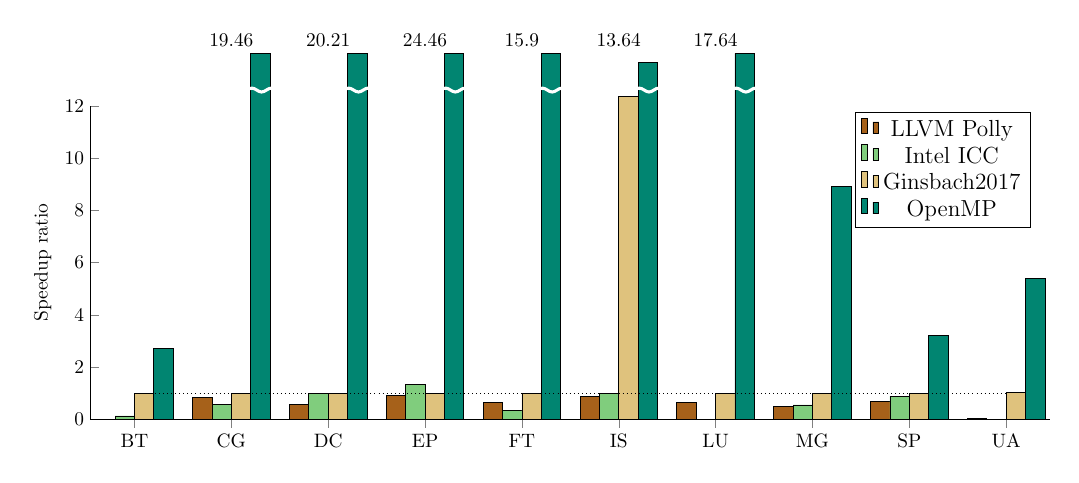
\begin{tikzpicture}[scale=0.70, every node/.style={transform shape}] 
    \begin{axis}[
      every axis plot post/.style={/pgf/number format/fixed},
      ylabel={Speedup ratio},
      legend style={font=\large},
      ybar=0pt,
      bar width=10pt,
      x=50pt,
      ymin=0,
      axis on top,
      ymax=12,
      xtick=data,
      enlarge x limits=0.05,
      symbolic x coords={BT,CG,DC,EP,FT,IS,LU,MG,SP,UA},
      restrict y to domain*=0:14, % Cut values off at 14
      visualization depends on=rawy\as\rawy, % Save the unclipped values
      after end axis/.code={ % Draw line indicating break
              \draw [ultra thick, white, decoration={snake, amplitude=1pt}, decorate] (rel axis cs:0,1.05) -- (rel axis cs:1,1.05);
              \draw [ultra thin, dotted] (axis cs:BT,1) -- (axis cs:UA,1);
          },
      axis lines*=left,
      clip=false
      ]
      \node[above] at (axis cs:CG,14) {19.46};
      \node[above] at (axis cs:DC,14) {20.21};
      \node[above] at (axis cs:EP,14) {24.46};
      \node[above] at (axis cs:FT,14) {15.9};
      \node[above] at (axis cs:IS,14) {13.64};
      \node[above] at (axis cs:LU,14) {17.64};
      \legend{LLVM Polly, Intel ICC, Ginsbach2017, OpenMP}
      \addplot[fill=Polly] coordinates {(BT,0) (CG,0.85) (DC,0.58) (EP,0.91) (FT,0.65) (IS,0.9) (LU,0.66) (MG,0.5) (SP,0.7) (UA,0.03)};
      \addplot[fill=ICC] coordinates {(BT,0.14) (CG,0.58) (DC,0.99) (EP,1.36) (FT,0.36) (IS,1) (LU,0.02) (MG,0.56) (SP,0.9) (UA,0)};
      \addplot[fill=Gins] coordinates {(BT,1) (CG,0.99) (DC,1) (EP,1) (FT,1) (IS,12.36) (LU,1) (MG,1) (SP,1) (UA,1.03)};
      \addplot[fill=OMP] coordinates {(BT,2.72) (CG,19.46) (DC,20.21) (EP,24.46) (FT,15.9) (IS,13.64) (LU,17.64) (MG,8.9) (SP,3.22) (UA,5.38)};
    \end{axis}
  \end{tikzpicture}
\end{figure}

\end{document}
